\chapter{Solution Overview \\
  \small{\textit{-- Evan Ciok, Sophia DiCuffa, Carson McManus}}
  \index{Chapter!solution}
  \index{load balancing}
  \index{load balancer}
  \label{Chapter::SolutionOverview}}

\section{Current Architecture}

The Monolith's \index{Monolith} current internals is shown in Figure \ref{Figure::monolith-class-current}.

\begin{figure}[!h]
  \centering
  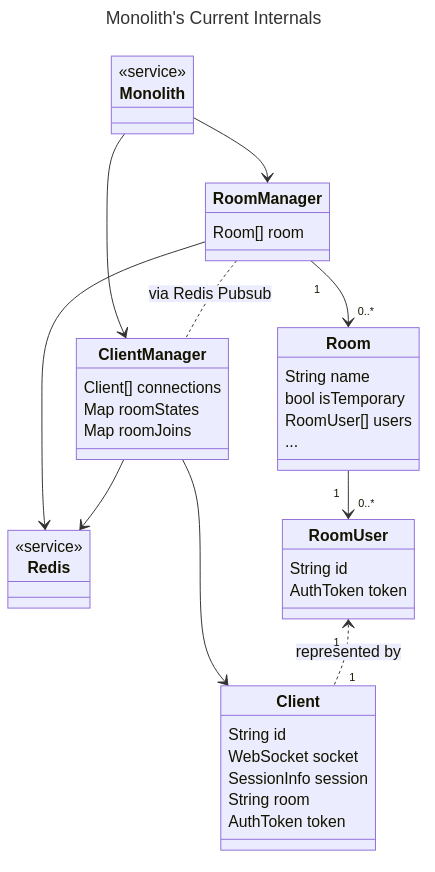
\includegraphics[width=0.4\textwidth]{Figures/monolith-class-current.png}
  \caption{Class diagram for the Monolith's current internals}
  \label{Figure::monolith-class-current}
\end{figure}

It suffers from years of ad-hoc development, and is not designed to scale. It's riddled with technical debt from previous attempts at horizontal scaling \index{horizontal scaling}. In it's current state, it is not possible to add more monoliths without causing room synchronization issues. The solution to this problem is to use a load balancer \index{load balancer}.

\section{A Smart Load Balancer}

The solution to scaling OTT is to use a load balancer. The Balancer will be an optional, seperate component that would be deployed alongside the Monoliths.

\subsection{What is a load balancer?}

A load balancer is a server that distributes load across multiple servers. It is a common solution to the problem of scaling a web application.

The load balancer must be able to:
\begin{itemize}
  \item Distribute load across multiple Monoliths
  \item Forward HTTP requests to the correct Monolith
  \item Send WebSocket messages to the correct Monolith
\end{itemize}

These requirements imply that a normal HTTP load balancer (like nginx) will not work, and the need for a specialized implementation. The specifics of how the load balancer will work will be discussed in the following chapters.

\section{New Architecture}

With the load balancer, OTT's architecture will look like this: Figure \ref{Figure::deployment-new}

\begin{figure}[!h]
  \centering
  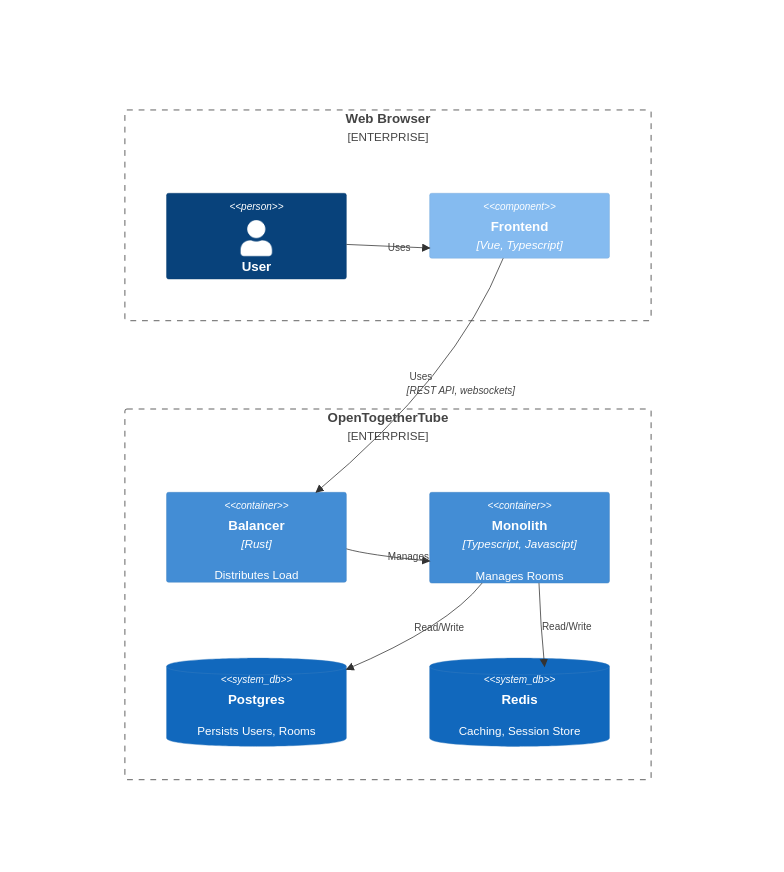
\includegraphics[width=1\textwidth]{Figures/deployment-new.png}
  \caption{High level overview of OTT's new architecture with a load balancer}
  \label{Figure::deployment-new}
\end{figure}

Figure \ref{Figure::monolith-class-new} shows what the Monolith's internals will look like after we take into account the load balancer.

\begin{figure}[!h]
  \centering
  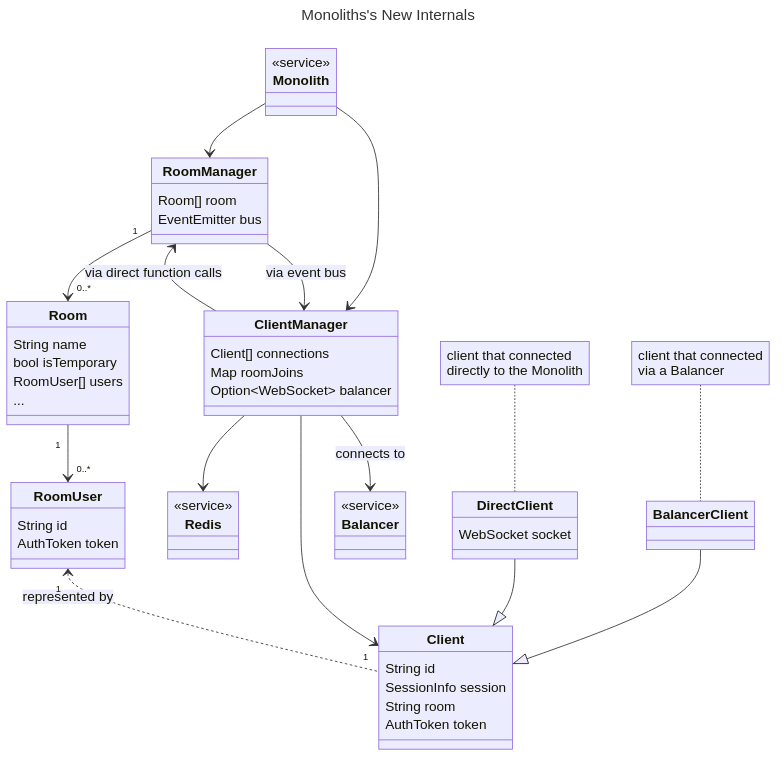
\includegraphics[width=0.8\textwidth]{Figures/monolith-class-new.png}
  \caption{The Monolith's new internals}
  \label{Figure::monolith-class-new}
\end{figure}

Note how the connection to the balancer is optional. The main differences between this and figure \ref{Figure::monolith-class-current} are:
\begin{enumerate}
  \item that Monoliths now have 2 types of clients representing how the client is connecting to the Monolith.
  \item that the RoomManager and ClientManager no longer communicate through Redis.
\end{enumerate}